\section{Model Structure}

\subsection{General features}

Our COVID-19 model is a series of compartments representing transitions between states relevant to infection with SARS-CoV-2 and onward transmission of this virus.
Unlike previous iterations of this model (including our past publications on the epidemics in the Philippines, Malaysia and Victoria, Australia), our current model considers only states relevant to transmission.
Hospitalisation, admission to ICU and death are no longer represented as explicit model states, but are now calculated from model outputs through a convolution process.
The rationale for this approach is that the explicitly modelled states are reserved to represent considerations relevant to epidemic transmission dynamics only.
The other outcomes can be calculated from the quantities that are tracked during the process of numerically solving the dynamic system (``derived outputs'').
It should be noted that this is done after each model realisation, such that these quantities can still be compared to empirically observed outcomes and so used for calibration.

\subsection{Compartments}
Model compartments represent sequential progressions through the processes of infection with, progression through and recovery from the phases of SARS-CoV-2.
Reinfection is permitted in our model code structure, which is represented as transition from the recovered compartments back to the first infected compartment.
The following compartments are implemented:
\begin{itemize}
    \item Susceptible
    \begin{itemize}
        \item Persons never previously infected with SARS-CoV-2 during the model simulation period
    \end{itemize}
    \item Latent
    \begin{itemize}
        \item Persons recently infected with SARS-CoV-2, but not yet infectious
        \item This compartment is divided into two sequential phases
    \end{itemize}
    \item Infectious
    \begin{itemize}
        \item Persons with active COVID-19 who are potentially infectious to others
        \item This compartment is divided into two sequential phases
        \item The second of these two sequential compartments includes any persons who are identified through the health system and asked to isolate
        \item The infectiousness of the second compartment will be reduced to capture the effect of case isolation
    \end{itemize}
    \item Recovered
    \begin{itemize}
        \item Persons recovered from COVID-19 during the model simulation period
        \item This compartment is divided into two sequential phases
        \item Reinfection from these compartments is permitted and will occur at a different rate for the two sequential phases
        \item This compartment retains the stratification by strain (or variant of concern (``VoC'')), with the strain of the last infection episode used for classification
    \end{itemize}
\end{itemize}


\begin{figure}[ht]
    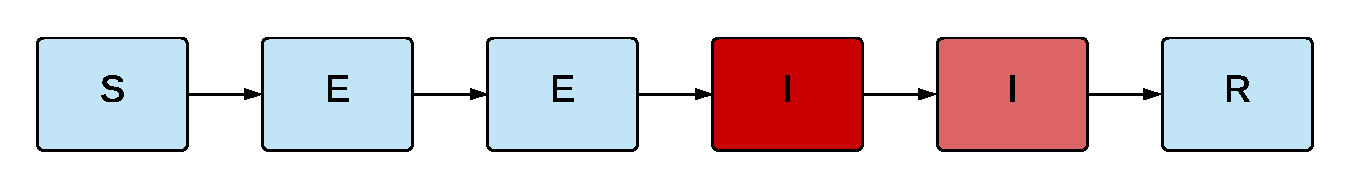
\includegraphics[width=\textwidth]{../tex_descriptions/models/sm_sir/sm_sir_seir.pdf}
    \caption[Unstratified compartmental model structure.]{Unstratified compartmental model structure. \small S = susceptible, E = exposed, I = active, R = recovered/removed. Depth of pink/red shading indicates the infectiousness of the compartment.}
    \label{fig:seeiir}
\end{figure}
